% -*- coding: utf-8 -*-
% Aula: Programacao dinamica -- memoization e subestrutura otima
% Fontes principais: Cormen et al. (2009), cap. 15 (secs. 15.1 e 15.3);
% Kleinberg e Tardos (2006), secs. 6.1 e 6.2 (intervalos ponderados);
% Levitin (2012), cap. 8; Dasgupta et al. (2008), secs. 0.2 e 6.1.
% Material de partida: ~/work/archive/20260316-d75e5aa4/UFS_Beamer/progdim.tex
\documentclass[aspectratio=169,xcolor=table]{beamer}

\usetheme{UFS}

\usepackage[utf8]{inputenc}
\usepackage[T1]{fontenc}
\usepackage[brazil]{babel}
\usepackage{amsmath,amssymb,amsthm}
\usepackage{graphicx}
\usepackage{booktabs}
\usepackage{listings}
\usepackage{xcolor}
\usepackage{tikz}
\usetikzlibrary{arrows.meta, shapes, positioning, calc, fit, matrix,
  decorations.pathreplacing, decorations.pathmorphing, backgrounds, patterns}

\definecolor{codegreen}{rgb}{0,0.6,0}
\definecolor{codegray}{rgb}{0.5,0.5,0.5}
\definecolor{codepurple}{rgb}{0.58,0,0.82}
\definecolor{backcolour}{rgb}{0.95,0.95,0.92}

\lstdefinestyle{mystyle}{
    language=C,
    backgroundcolor=\color{backcolour},
    commentstyle=\color{codegreen},
    keywordstyle=\color{magenta},
    numberstyle=\tiny\color{codegray},
    stringstyle=\color{codepurple},
    breakatwhitespace=false,
    breaklines=true,
    captionpos=b,
    keepspaces=true,
    columns=fullflexible,
    numbers=none,
    showspaces=false,
    showstringspaces=false,
    showtabs=false,
    tabsize=2,
    frame=single,
    rulecolor=\color{gray},
    extendedchars=true,
    basicstyle=\ttfamily\scriptsize,
    literate={ê}{{\^e}}1 {à}{{\`a}}1 {ú}{{\'u}}1 {õ}{{\~o}}1 {ó}{{\'o}}1
             {í}{{\'i}}1 {á}{{\'a}}1 {ã}{{\~a}}1 {é}{{\'e}}1 {ç}{{\c{c}}}1
             {â}{{\^a}}1 {ô}{{\^o}}1 {ü}{{\"u}}1 {Á}{{\'A}}1 {É}{{\'E}}1
}
\lstset{style=mystyle}

% ---- estilos TikZ reutilizados ----
\tikzset{
  box/.style={rectangle, draw=blue!60, fill=blue!10, rounded corners,
              minimum width=6.2cm, minimum height=0.55cm, font=\scriptsize},
  fase/.style={rectangle, rounded corners, draw=blue!60, fill=blue!10,
               minimum width=2.3cm, minimum height=0.6cm, font=\scriptsize,
               align=center},
  fn/.style={circle, draw=blue!60!black, fill=blue!8, inner sep=0pt,
             minimum size=5.2mm, font=\tiny},
  rep3/.style={fn, fill=orange!35, draw=orange!80!black},
  rep2/.style={fn, fill=red!20, draw=red!70!black},
  vtx/.style={circle, draw=blue!60!black, fill=blue!8, inner sep=0pt,
              minimum size=6mm, font=\scriptsize},
  cel/.style={draw=gray!70, minimum width=7mm, minimum height=5mm, inner sep=0pt,
              font=\scriptsize},
  arc/.style={-{Stealth}, thick}
}

% intervalo da instancia condutora: \intervalo{linha}{inicio}{fim}{rotulo}{estilo}
\newcommand{\intervalo}[5]{%
  \draw[line width=2.4mm, #5] (#2,-#1*0.42) -- (#3,-#1*0.42);
  \node[font=\tiny, anchor=west] at (#3+0.1,-#1*0.42) {#4};%
}

% ---- ponteiro de leitura no rodape do frame ----
\newcommand{\fonte}[1]{%
  \vfill
  {\tiny\color{gray!55!black}\textbf{Para aprofundar:} #1\par}%
}

\title{Programação dinâmica}
\subtitle{Memoization e subestrutura ótima}
\author[André Y. Kashiwabara <andreyoshiaki@dcomp.ufs.br>]{Prof.\ Dr.\ André Yoshiaki Kashiwabara}
\institute{Departamento de Computação --- Universidade Federal de Sergipe}
\date{\today}

\begin{document}

\begin{frame}[plain,noframenumbering]
  \titlepage
\end{frame}

\begin{frame}{O que você vai aprender hoje}
  \begin{center}
  \begin{tikzpicture}[node distance=3mm]
    \node[box] (t1) {1.\ Subproblemas que se repetem: Fibonacci em $\Theta(\phi^n)$};
    \node[box, below=of t1] (t2) {2.\ Memoization e bottom-up: cada subproblema uma vez só};
    \node[box, below=of t2, fill=orange!20, draw=orange!80!black] (t3)
         {3.\ Subestrutura ótima: quando a PD está correta};
    \node[box, below=of t3] (t4) {4.\ Os quatro passos em um problema real: intervalos ponderados};
    \foreach \a/\b in {t1/t2, t2/t3, t3/t4}
      \draw[-{Stealth}, thick, blue!60!black] (\a) -- (\b);
    \draw[-{Stealth}, thick, orange!80!black, dashed]
      (t4.east) to[out=0, in=0, looseness=1.6]
      node[right, xshift=1mm, font=\tiny, align=left]
      {repetição $\Rightarrow$ eficiência\\subestrutura $\Rightarrow$ corretude} (t1.east);
  \end{tikzpicture}
  \end{center}
  \medskip
  {\scriptsize\centering
  Programação dinâmica (PD) = \textbf{recursão} + \textbf{tabela}. As duas condições para usá-la
  são os dois assuntos centrais desta aula.\par}
\end{frame}

% =====================================================================
\section{Subproblemas que se repetem}

\begin{frame}{Por que precisamos de algo além de divisão e conquista?}
  \begin{columns}[T]
    \begin{column}{0.48\textwidth}
      \textbf{Problema:}\\[2pt]
      \scriptsize Em divisão e conquista (Karatsuba, Strassen, par mais próximo), os
      subproblemas são \textbf{disjuntos}: cada metade é resolvida uma vez.
      \medskip

      Muitas recorrências, porém, geram subproblemas que se \textbf{sobrepõem}. A recursão
      direta resolve o mesmo subproblema muitas vezes e o tempo vira
      \textbf{exponencial}.
    \end{column}
    \begin{column}{0.48\textwidth}
      \textbf{Solução:}\\[2pt]
      \scriptsize Resolver cada subproblema distinto \textbf{uma única vez} e guardar a
      resposta em uma \textbf{tabela}. Na próxima vez que ele aparecer, basta consultar.
      \medskip

      Troca-se memória por tempo: se há poucos subproblemas distintos (polinomial), o
      algoritmo fica polinomial.
    \end{column}
  \end{columns}
  \fonte{Cormen et al.\ (2009), introdução do cap.~15~\cite{cormen2009introduction};
    Levitin (2012), introdução do cap.~8~\cite{levitin2012introduction}.}
\end{frame}

\begin{frame}[fragile]{Fibonacci pela definição}
  \begin{columns}[T]
    \begin{column}{0.4\textwidth}
      \scriptsize $F_0=0,\quad F_1=1,\quad F_n = F_{n-1}+F_{n-2}.$
\begin{lstlisting}
long fib( int n) {
   if (n <= 1) return n;
   return fib( n-1) + fib( n-2);
}
\end{lstlisting}
      \scriptsize A árvore ao lado é a de \texttt{fib(5)}: 15 chamadas para 6 valores
      distintos. $F_3$ é calculado \textcolor{orange!80!black}{\textbf{2 vezes}},
      $F_2$ \textcolor{red!70!black}{\textbf{3 vezes}}.
    \end{column}
    \begin{column}{0.58\textwidth}
      \centering
      \begin{tikzpicture}[level distance=8.5mm,
          level 1/.style={sibling distance=36mm},
          level 2/.style={sibling distance=18mm},
          level 3/.style={sibling distance=9mm},
          level 4/.style={sibling distance=6mm},
          edge from parent/.style={draw, gray}]
        \node[fn] {$F_5$}
          child {node[fn] {$F_4$}
            child {node[rep3] {$F_3$}
              child {node[rep2] {$F_2$} child {node[fn] {$F_1$}} child {node[fn] {$F_0$}}}
              child {node[fn] {$F_1$}}}
            child {node[rep2] {$F_2$} child {node[fn] {$F_1$}} child {node[fn] {$F_0$}}}}
          child {node[rep3] {$F_3$}
            child {node[rep2] {$F_2$} child {node[fn] {$F_1$}} child {node[fn] {$F_0$}}}
            child {node[fn] {$F_1$}}};
      \end{tikzpicture}
    \end{column}
  \end{columns}
  \fonte{Dasgupta et al.\ (2008), \S 0.2~\cite{dasgupta2008algorithms};
    Levitin (2012), introdução do cap.~8~\cite{levitin2012introduction}.}
\end{frame}

\begin{frame}{Quantas chamadas faz \texttt{fib(n)}?}
  \begin{columns}[c]
    \begin{column}{0.5\textwidth}
      \scriptsize Seja $C(n)$ o número de chamadas:
      \[ C(0)=C(1)=1, \qquad C(n) = C(n-1) + C(n-2) + 1. \]
      Por indução, $C(n) = 2F_{n+1}-1$. Como $F_n \approx \phi^n/\sqrt5$, com
      $\phi = \frac{1+\sqrt5}{2}\approx 1{,}618$:
      \[ C(n) \in \Theta(\phi^n). \]
      O tempo cresce \textbf{como a própria resposta}: só há 6 valores distintos em
      \texttt{fib(5)}, mas o algoritmo faz $2F_6-1=15$ chamadas.
    \end{column}
    \begin{column}{0.44\textwidth}
      \centering\scriptsize
      \begin{tabular}{rrr}
        \toprule
        $n$ & chamadas $C(n)$ & distintos \\
        \midrule
        5  & 15 & 6 \\
        10 & 177 & 11 \\
        20 & 21\,891 & 21 \\
        30 & 2\,692\,537 & 31 \\
        40 & 331\,160\,281 & 41 \\
        50 & $\approx 4\cdot 10^{10}$ & 51 \\
        \bottomrule
      \end{tabular}
      \medskip

      A $10^9$ chamadas/s, \texttt{fib(50)} leva $\approx 40$\,s;
      \texttt{fib(70)}, mais de um dia.
    \end{column}
  \end{columns}
  \fonte{Dasgupta et al.\ (2008), \S 0.2~\cite{dasgupta2008algorithms};
    Cormen et al.\ (2009), Exercícios 3.2-6 e 3.2-7 (razão áurea)~\cite{cormen2009introduction}.}
\end{frame}

\begin{frame}{Subproblemas sobrepostos: definição}
  \begin{columns}[c]
    \begin{column}{0.52\textwidth}
      \begin{block}{Definição}
        \scriptsize Um problema tem \alert{subproblemas sobrepostos} quando um algoritmo
        recursivo para ele resolve \textbf{os mesmos subproblemas repetidamente}, em vez de
        gerar sempre subproblemas novos. Interessa o caso em que o número de subproblemas
        \emph{distintos} é polinomial no tamanho da entrada.
      \end{block}
      \begin{exampleblock}{Intuição}
        \scriptsize Desenhe cada subproblema \emph{uma vez} e ligue-o aos que ele usa: em
        D\&C sai uma \textbf{árvore}; em PD, um \textbf{DAG} pequeno.
      \end{exampleblock}
    \end{column}
    \begin{column}{0.44\textwidth}
      \centering
      \begin{tikzpicture}[node distance=4mm and 3mm]
        \node[font=\tiny\bfseries] at (0,0.55) {D\&C: subproblemas disjuntos};
        \node[fn] (r) at (0,0) {$n$};
        \node[fn] (a) at (-0.9,-0.8) {$\frac n2$};
        \node[fn] (b) at (0.9,-0.8) {$\frac n2$};
        \foreach \x in {-1.35,-0.45} \draw[gray] (a) -- (\x,-1.45) node[fn, below] {$\frac n4$};
        \foreach \x in {0.45,1.35} \draw[gray] (b) -- (\x,-1.45) node[fn, below] {$\frac n4$};
        \draw[gray] (r) -- (a); \draw[gray] (r) -- (b);
        \begin{scope}[yshift=-3.1cm]
          \node[font=\tiny\bfseries] at (0,0.85) {PD: grafo de subproblemas de \texttt{fib(5)}};
          \foreach \i in {5,...,0}
            \node[fn] (f\i) at ({(5-\i)*0.9-2.25},0) {$F_{\i}$};
          \foreach \i/\j in {5/4,4/3,3/2,2/1,1/0}
            \draw[arc, blue!60!black] (f\i) -- (f\j);
          \foreach \i/\j in {5/3,4/2,3/1,2/0}
            \draw[arc, orange!80!black] (f\i) to[bend left=55] (f\j);
        \end{scope}
      \end{tikzpicture}
    \end{column}
  \end{columns}
  \fonte{Cormen et al.\ (2009), \S 15.3, ``Overlapping subproblems'' e \S 15.1, ``Subproblem
    graphs''~\cite{cormen2009introduction}.}
\end{frame}

\begin{frame}{Por que ``programação dinâmica''?}
  \begin{columns}[c]
    \begin{column}{0.72\textwidth}
      \scriptsize
      \begin{itemize}\scriptsize
        \item Richard Bellman formulou o método nos anos 1950, na RAND Corporation, para
              problemas de decisão em vários estágios; o livro \emph{Dynamic Programming}
              é de 1957.
        \item ``Programação'' tem o sentido de \textbf{planejamento} preenchendo uma
              \textbf{tabela} (como em ``programação linear''), não de escrever código.
        \item Segundo a autobiografia de Bellman, o nome foi escolhido para soar bem a um
              secretário de Defesa avesso à palavra ``pesquisa'': ``dinâmica'' indicava
              estágios e tempo, e era difícil de usar em sentido pejorativo.
        \item A ideia reaparece em toda a disciplina: Bellman-Ford, Floyd-Warshall, mochila,
              LCS e alinhamento de sequências em bioinformática.
      \end{itemize}
    \end{column}
    \begin{column}{0.24\textwidth}
      \centering
      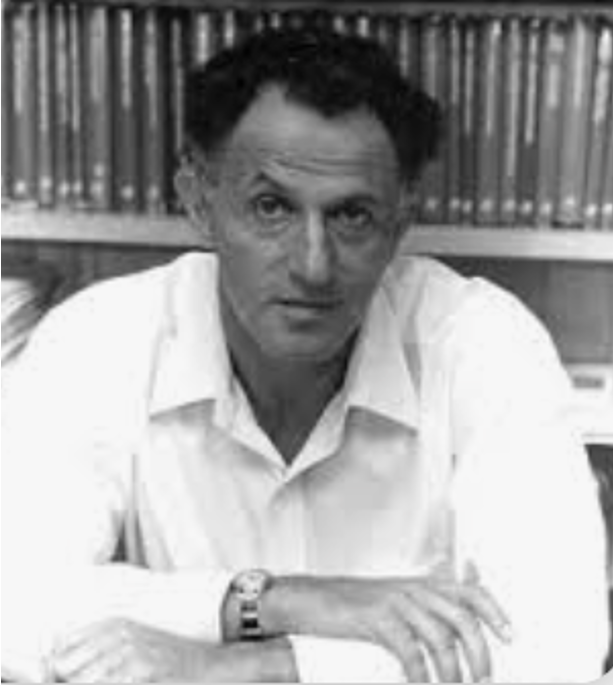
\includegraphics[width=0.9\textwidth]{Bellman.png}\\[2pt]
      {\tiny Richard Bellman (1920--1984)\\ Imagem: Wikimedia Commons}
    \end{column}
  \end{columns}
  \fonte{Bellman (1957)~\cite{bellman1957dynamic}; Dreyfus (2002)~\cite{dreyfus2002richard};
    Cormen et al.\ (2009), notas do cap.~15~\cite{cormen2009introduction}.}
\end{frame}

\begin{frame}{Recapitulando: subproblemas que se repetem}
  \begin{block}{O que aprendemos}
    \begin{itemize}\scriptsize
      \item A recursão direta de Fibonacci faz $2F_{n+1}-1 \in \Theta(\phi^n)$ chamadas,
            mas só existem $n+1$ subproblemas distintos.
      \item \textbf{Subproblemas sobrepostos}: a recursão volta aos mesmos subproblemas;
            o grafo de subproblemas é um DAG pequeno, não uma árvore enorme.
      \item Divisão e conquista: subproblemas disjuntos. PD: subproblemas compartilhados,
            resolvidos uma vez e guardados em tabela.
    \end{itemize}
  \end{block}
  \fonte{Cormen et al.\ (2009), \S 15.3~\cite{cormen2009introduction}.}
\end{frame}

% =====================================================================
\section{Memoization e bottom-up}

\begin{frame}{Por que guardar respostas?}
  \begin{columns}[T]
    \begin{column}{0.48\textwidth}
      \textbf{Problema:}\\[2pt]
      \scriptsize A recorrência $F_n = F_{n-1}+F_{n-2}$ está \textbf{correta}; o problema é
      só a repetição. Reescrever o algoritmo do zero dá trabalho e pode introduzir erros.
    \end{column}
    \begin{column}{0.48\textwidth}
      \textbf{Solução:} duas formas de aproveitar a mesma recorrência.\\[2pt]
      \scriptsize
      \begin{itemize}\scriptsize
        \item \textbf{Top-down com memoization}: mantém a recursão e anota cada resposta
              na tabela antes de devolvê-la.
        \item \textbf{Bottom-up}: preenche a tabela em uma ordem em que cada entrada só
              depende de entradas já preenchidas.
      \end{itemize}
      Ambas fazem $\Theta(n)$ trabalho para Fibonacci.
    \end{column}
  \end{columns}
  \fonte{Cormen et al.\ (2009), \S 15.1, ``Top-down with memoization'' e ``Bottom-up
    method''~\cite{cormen2009introduction}.}
\end{frame}

\begin{frame}[fragile]{Memoization: definição}
  \begin{columns}[T]
    \begin{column}{0.47\textwidth}
      \begin{block}{Definição}
        \scriptsize Um algoritmo recursivo \alert{memoizado} guarda em uma tabela a resposta
        de cada subproblema na primeira vez que a calcula. Antes de calcular, consulta a
        tabela: se a resposta já está lá, devolve-a sem recursão.
      \end{block}
      \begin{exampleblock}{Intuição}
        \scriptsize Um ``memorando'' para si mesmo: o termo \emph{memo function} é de
        Michie (1968), daí \emph{memoization}, sem ``r''.
      \end{exampleblock}
    \end{column}
    \begin{column}{0.5\textwidth}
\begin{lstlisting}
long memo[MAX];  /* inicializado com -1 */

long fibMemo( int n) {
   if (memo[n] >= 0)       /* já calculado? */
      return memo[n];
   long r;
   if (n <= 1) r = n;
   else r = fibMemo( n-1) + fibMemo( n-2);
   memo[n] = r;            /* anota */
   return r;
}
\end{lstlisting}
      \scriptsize Cada $F_k$ é calculado uma vez: $2n-1$ chamadas, $\Theta(n)$.
    \end{column}
  \end{columns}
  \fonte{Cormen et al.\ (2009), \S 15.3, ``Memoization''~\cite{cormen2009introduction};
    Michie (1968)~\cite{michie1968memo}.}
\end{frame}

\begin{frame}[fragile]{Bottom-up: a tabela na ordem do DAG}
  \begin{columns}[T]
    \begin{column}{0.47\textwidth}
\begin{lstlisting}
long fibBU( int n) {
   long F[MAX];
   F[0] = 0;  F[1] = 1;
   for (int k = 2; k <= n; ++k)
      F[k] = F[k-1] + F[k-2];
   return F[n];
}
\end{lstlisting}
      \scriptsize Sem recursão, sem pilha, sem teste ``já calculei?''. Como $F[k]$ só usa as
      duas entradas anteriores, dá para guardar só duas variáveis: espaço $O(1)$.
    \end{column}
    \begin{column}{0.49\textwidth}
      \centering
      \begin{tikzpicture}
        \foreach \v [count=\i from 0] in {0,1,1,2,3,5,8} {
          \node[cel, fill=blue!8] (c\i) at (\i*0.75,0) {\v};
          \node[font=\tiny, gray] at (\i*0.75,0.45) {$\i$};
        }
        \node[cel, fill=orange!30] at (5*0.75,0) {5};
        \draw[arc, orange!80!black] (c4.south) to[bend right=40] (c5.south);
        \draw[arc, orange!80!black] (c3.south) to[bend right=50] (c5.south);
        \draw[arc, gray] (-0.2,-0.9) -- node[below, font=\tiny] {ordem de preenchimento: ordem topológica inversa do DAG} (4.7,-0.9);
      \end{tikzpicture}
      \medskip

      \scriptsize
      \begin{tabular}{lcc}
        \toprule
        & top-down memo & bottom-up \\
        \midrule
        ordem & a recursão decide & você decide \\
        subproblemas & só os necessários & todos \\
        custo extra & pilha + testes & nenhum \\
        \bottomrule
      \end{tabular}
    \end{column}
  \end{columns}
  \fonte{Cormen et al.\ (2009), \S 15.1, ``Subproblem graphs''~\cite{cormen2009introduction};
    Dasgupta et al.\ (2008), \S 6.1~\cite{dasgupta2008algorithms}.}
\end{frame}

\begin{frame}{Exemplo: rastreando \texttt{fibMemo(5)}}
  \begin{columns}[c]
    \begin{column}{0.5\textwidth}
      \centering
      \begin{tikzpicture}[level distance=8mm, sibling distance=13mm,
          edge from parent/.style={draw, gray}]
        \node[fn] {$F_5$}
          child {node[fn] {$F_4$}
            child {node[fn] {$F_3$}
              child {node[fn] {$F_2$} child {node[fn] {$F_1$}} child {node[fn] {$F_0$}}}
              child {node[fn, fill=green!25, draw=green!50!black] {$F_1$}}}
            child {node[fn, fill=green!25, draw=green!50!black] {$F_2$}}}
          child {node[fn, fill=green!25, draw=green!50!black] {$F_3$}};
      \end{tikzpicture}
    \end{column}
    \begin{column}{0.46\textwidth}
      \begin{exampleblock}{Exemplo}
        \scriptsize
        \begin{itemize}\scriptsize
          \item A recursão desce pelo ramo esquerdo até $F_1$ e $F_0$ e anota
                $F_2, F_3, F_4$ na volta.
          \item Os nós \textcolor{green!50!black}{\textbf{verdes}} são consultas à tabela:
                devolvem na hora, sem filhos.
          \item Total: 9 chamadas (antes eram 15). Para $n$ geral, $2n-1$ chamadas
                contra $2F_{n+1}-1$.
        \end{itemize}
      \end{exampleblock}
    \end{column}
  \end{columns}
  \fonte{Cormen et al.\ (2009), \S 15.1, \textsc{Memoized-Cut-Rod}~\cite{cormen2009introduction};
    Dasgupta et al.\ (2008), \S 6.1~\cite{dasgupta2008algorithms}.}
\end{frame}

\begin{frame}{Recapitulando: memoization e bottom-up}
  \begin{block}{O que aprendemos}
    \begin{itemize}\scriptsize
      \item \textbf{Memoization}: mesma recursão, mais uma tabela consultada antes e
            preenchida depois de cada cálculo.
      \item \textbf{Bottom-up}: laço que preenche a tabela em ordem topológica inversa do
            grafo de subproblemas.
      \item Tempo $\approx$ (nº de subproblemas distintos) $\times$ (trabalho por
            subproblema). Fibonacci: $(n+1)\times O(1) = \Theta(n)$.
      \item As duas versões têm o mesmo tempo assintótico; a recorrência é que precisa
            estar certa.
    \end{itemize}
  \end{block}
  \fonte{Cormen et al.\ (2009), \S 15.1 e \S 15.3~\cite{cormen2009introduction}.}
\end{frame}

% =====================================================================
\section{Subestrutura ótima}

\begin{frame}{Por que nem todo problema de otimização serve?}
  \begin{columns}[T]
    \begin{column}{0.48\textwidth}
      \textbf{Problema:}\\[2pt]
      \scriptsize Em Fibonacci só há \emph{um} jeito de combinar as respostas: somar.
      Em problemas de \textbf{otimização} (mínimo, máximo), a recorrência escolhe a
      melhor entre várias opções, usando as respostas \emph{ótimas} dos subproblemas.
      \medskip

      Isso só é correto se a solução ótima for feita de pedaços ótimos.
    \end{column}
    \begin{column}{0.48\textwidth}
      \textbf{Solução:}\\[2pt]
      \scriptsize Antes de escrever a recorrência, \textbf{provar} que o problema tem
      \textbf{subproblemas sobrepostos} e \textbf{subestrutura ótima}, as duas
      condições que Cormen et al.\ citam para a PD funcionar.
      \medskip

      A primeira dá a \textbf{eficiência}; a segunda, a \textbf{corretude}.
      É o mesmo papel do invariante de laço da Unidade 1.
    \end{column}
  \end{columns}
  \fonte{Cormen et al.\ (2009), \S 15.3, ``Elements of dynamic programming''~\cite{cormen2009introduction}.}
\end{frame}

\begin{frame}{Subestrutura ótima: definição}
  \begin{columns}[c]
    \begin{column}{0.5\textwidth}
      \begin{block}{Definição}
        \scriptsize Um problema tem \alert{subestrutura ótima} se toda solução ótima do
        problema contém soluções ótimas dos subproblemas que ela usa.
      \end{block}
      \begin{exampleblock}{Intuição: o argumento ``recorta e cola''}
        \scriptsize Suponha que a solução ótima usa uma solução $S'$ \emph{não ótima} de um
        subproblema. Recorte $S'$ e cole no lugar uma solução melhor. O resultado é melhor
        que o ótimo: contradição.
      \end{exampleblock}
    \end{column}
    \begin{column}{0.46\textwidth}
      \centering
      \begin{tikzpicture}
        \node[vtx] (u) at (0,0) {$u$};
        \node[vtx] (x) at (2.2,0) {$x$};
        \node[vtx] (v) at (4.2,0) {$v$};
        \draw[arc, blue!60!black, decorate, decoration={snake, amplitude=0.6mm, segment length=3mm, post length=1.5mm}]
          (u) -- node[below=1mm, font=\tiny] {$p_{ux}$} (x);
        \draw[arc, blue!60!black, decorate, decoration={snake, amplitude=0.6mm, segment length=3mm, post length=1.5mm}]
          (x) -- node[below=1mm, font=\tiny] {$p_{xv}$} (v);
        \draw[arc, green!50!black, dashed, thick] (u) to[bend left=45]
          node[above, font=\tiny] {$p'_{ux}$ mais curto?} (x);
        \node[font=\tiny, align=center] at (2.1,-1.1)
          {Se $p'_{ux}$ fosse mais curto que $p_{ux}$, \\
           $p'_{ux}\,p_{xv}$ seria mais curto que o caminho mínimo $u \leadsto v$.};
      \end{tikzpicture}
      \medskip

      {\scriptsize Logo, todo subcaminho de um caminho mínimo é mínimo.}
    \end{column}
  \end{columns}
  \fonte{Cormen et al.\ (2009), \S 15.3, ``Optimal substructure'', e Lema 24.1~\cite{cormen2009introduction}.}
\end{frame}

\begin{frame}{Contraexemplo: caminho simples mais longo}
  \begin{columns}[c]
    \begin{column}{0.36\textwidth}
      \centering
      \begin{tikzpicture}[node distance=17mm]
        \node[vtx] (q) {$q$};
        \node[vtx, right=of q] (r) {$r$};
        \node[vtx, below=of q] (s) {$s$};
        \node[vtx, below=of r] (t) {$t$};
        \foreach \a/\b in {q/r, q/s, r/t, s/t}
          \draw[{Stealth}-{Stealth}, thick, gray] (\a) -- (\b);
      \end{tikzpicture}
    \end{column}
    \begin{column}{0.6\textwidth}
      \scriptsize
      \begin{itemize}\scriptsize
        \item Caminho simples \textbf{mais longo} de $q$ a $t$: $q\to r\to t$ (ou
              $q\to s\to t$), com 2 arestas.
        \item O subcaminho $q\to r$ \textbf{não} é o mais longo de $q$ a $r$: esse é
              $q\to s\to t\to r$.
        \item O mais longo de $r$ a $t$ é $r\to q\to s\to t$. Juntar os dois ótimos dá
              $q\to s\to t\to r\to q\to s\to t$: \textbf{nem é simples}.
        \item Os subproblemas não são \textbf{independentes}: os vértices usados em um
              proíbem o outro. Sem subestrutura ótima, não há recorrência correta.
      \end{itemize}
      \smallskip
      Já o caminho \textbf{mínimo} tem subestrutura ótima (frame anterior): veremos PD para
      ele em Warshall-Floyd.
    \end{column}
  \end{columns}
  \fonte{Cormen et al.\ (2009), \S 15.3, Figura 15.6~\cite{cormen2009introduction}.}
\end{frame}

\begin{frame}{Os quatro passos da programação dinâmica}
  \begin{center}
  \begin{tikzpicture}[node distance=5mm and 7mm, fase/.append style={minimum width=2.9cm,
      minimum height=1.05cm, text width=2.7cm}]
    \node[fase] (p1) {\textbf{1. Estrutura}\\caracterizar a solução ótima};
    \node[fase, right=of p1] (p2) {\textbf{2. Recorrência}\\definir o valor ótimo recursivamente};
    \node[fase, right=of p2] (p3) {\textbf{3. Tabela}\\calcular o valor (memo ou bottom-up)};
    \node[fase, right=of p3, fill=green!12, draw=green!50!black] (p4)
         {\textbf{4. Solução}\\reconstruir a escolha ótima};
    \foreach \a/\b in {p1/p2, p2/p3, p3/p4} \draw[arc] (\a) -- (\b);
    \node[below=of p1, font=\tiny, align=center, text width=2.9cm] {subestrutura ótima:
      prova por recorta e cola};
    \node[below=of p2, font=\tiny, align=center, text width=2.9cm] {casos da \emph{última
      decisão} + caso base};
    \node[below=of p3, font=\tiny, align=center, text width=2.9cm] {tempo = nº de
      subproblemas $\times$ trabalho por subproblema};
    \node[below=of p4, font=\tiny, align=center, text width=2.9cm] {refaz as escolhas
      consultando a tabela; dispensável se só o valor interessa};
  \end{tikzpicture}
  \end{center}
  \fonte{Cormen et al.\ (2009), introdução do cap.~15~\cite{cormen2009introduction};
    Kleinberg e Tardos (2006), \S 6.2~\cite{kleinberg2006algorithm}.}
\end{frame}

\begin{frame}{Recapitulando: subestrutura ótima}
  \begin{block}{O que aprendemos}
    \begin{itemize}\scriptsize
      \item \textbf{Subestrutura ótima}: a solução ótima contém soluções ótimas de
            subproblemas. Prova típica: recorta e cola, por contradição.
      \item Caminho mínimo tem; caminho simples mais longo não tem (subproblemas
            dependentes).
      \item Subproblemas sobrepostos dão eficiência; subestrutura ótima dá corretude.
            A PD precisa das duas.
      \item Roteiro: estrutura $\to$ recorrência $\to$ tabela $\to$ reconstrução.
    \end{itemize}
  \end{block}
  \fonte{Cormen et al.\ (2009), \S 15.3~\cite{cormen2009introduction}.}
\end{frame}

% =====================================================================
\section{Seleção de intervalos ponderados}

\begin{frame}{Por que precisamos de PD para escolher intervalos?}
  \begin{columns}[T]
    \begin{column}{0.48\textwidth}
      \textbf{Problema:}\\[2pt]
      \scriptsize Um auditório recebe $n$ pedidos de reserva. O pedido $j$ ocupa o
      intervalo $[s_j, f_j)$ e paga $v_j$. Dois pedidos sobrepostos não podem ser
      aceitos juntos. Quais aceitar para \textbf{maximizar a receita}?
      \medskip

      Força bruta testa os $2^n$ subconjuntos.
    \end{column}
    \begin{column}{0.48\textwidth}
      \textbf{Solução:}\\[2pt]
      \scriptsize Com todos os pesos iguais, o guloso ``termina mais cedo'' é ótimo
      (Kleinberg e Tardos, \S 4.1). Com pesos, \textbf{nenhum guloso natural funciona}.
      \medskip

      Vamos aplicar os quatro passos e obter um algoritmo $O(n \log n)$.
    \end{column}
  \end{columns}
  \fonte{Kleinberg e Tardos (2006), \S 6.1~\cite{kleinberg2006algorithm}.}
\end{frame}

\begin{frame}{Intervalos ponderados: definição}
  \begin{columns}[c]
    \begin{column}{0.47\textwidth}
      \begin{block}{Definição}
        \scriptsize Entrada: intervalos $1,\dots,n$ ordenados por término,
        $f_1 \le \dots \le f_n$, com valores $v_j > 0$. Saída: um conjunto de intervalos
        \textbf{dois a dois disjuntos} com soma de valores máxima.
      \end{block}
      \begin{exampleblock}{O vetor $p$}
        \scriptsize $p(j)$ = maior índice $i < j$ com $f_i \le s_j$ (o último intervalo
        compatível com $j$); $p(j)=0$ se não houver.
        Na instância ao lado: $p = (0,0,1,0,3,3)$.
      \end{exampleblock}
    \end{column}
    \begin{column}{0.5\textwidth}
      \centering
      \begin{tikzpicture}[x=5.2mm]
        \draw[gray!50] (0,-0.1) -- (0,-2.75);
        \foreach \t in {0,2,...,10} {
          \draw[gray!30] (\t,-0.1) -- (\t,-2.75);
          \node[font=\tiny, gray] at (\t,0.1) {\t};
        }
        \intervalo{1}{0}{4}{$1$: $v{=}1$, $p{=}0$}{blue!45}
        \intervalo{2}{1}{6}{$2$: $v{=}6$, $p{=}0$}{blue!45}
        \intervalo{3}{5}{7}{$3$: $v{=}4$, $p{=}1$}{blue!45}
        \intervalo{4}{2}{9}{$4$: $v{=}7$, $p{=}0$}{blue!45}
        \intervalo{5}{8}{10}{$5$: $v{=}2$, $p{=}3$}{blue!45}
        \intervalo{6}{7}{11}{$6$: $v{=}1$, $p{=}3$}{blue!45}
      \end{tikzpicture}
    \end{column}
  \end{columns}
  \fonte{Kleinberg e Tardos (2006), \S 6.1, Figura 6.2~\cite{kleinberg2006algorithm}.}
\end{frame}

\begin{frame}{Exemplo: os gulosos falham nesta instância}
  \begin{columns}[c]
    \begin{column}{0.5\textwidth}
      \centering
      \begin{tikzpicture}[x=5.2mm]
        \foreach \t in {0,2,...,10} {
          \draw[gray!30] (\t,-0.1) -- (\t,-2.75);
          \node[font=\tiny, gray] at (\t,0.1) {\t};
        }
        \intervalo{1}{0}{4}{$1$: $1$}{orange!60}
        \intervalo{2}{1}{6}{$2$: $6$}{green!55!black}
        \intervalo{3}{5}{7}{$3$: $4$}{orange!60}
        \intervalo{4}{2}{9}{$4$: $7$}{red!45}
        \intervalo{5}{8}{10}{$5$: $2$}{green!55!black}
        \intervalo{6}{7}{11}{$6$: $1$}{gray!40}
      \end{tikzpicture}
    \end{column}
    \begin{column}{0.46\textwidth}
      \begin{exampleblock}{Exemplo}
        \scriptsize
        \begin{tabular}{lll}
          \toprule
          critério & escolhe & valor \\
          \midrule
          \textcolor{orange!80!black}{termina mais cedo} & $\{1,3,5\}$ & $1+4+2=7$ \\
          \textcolor{red!70!black}{maior valor} & $\{4\}$ & $7$ \\
          \textcolor{green!50!black}{ótimo} & $\{2,5\}$ & $6+2=\mathbf{8}$ \\
          \bottomrule
        \end{tabular}
        \medskip

        Cada guloso decide olhando um intervalo de cada vez. O ótimo depende de
        \textbf{combinações}: é isso que a tabela vai registrar.
      \end{exampleblock}
    \end{column}
  \end{columns}
  \fonte{Kleinberg e Tardos (2006), \S 6.1~\cite{kleinberg2006algorithm}.}
\end{frame}

\begin{frame}{Passo 1: a estrutura de uma solução ótima}
  \scriptsize Seja $O_j$ uma solução ótima para os intervalos $\{1,\dots,j\}$ e
  $\mathrm{OPT}(j)$ o seu valor. Olhe para a \textbf{última decisão}: o intervalo $j$ está
  ou não está em $O_j$.
  \medskip

  \begin{columns}[T]
    \begin{column}{0.48\textwidth}
      \begin{block}{Caso $j \notin O_j$}
        \scriptsize $O_j$ é solução para $\{1,\dots,j-1\}$ e precisa ser \textbf{ótima} para
        esse subproblema; senão, troque-a por uma melhor (recorta e cola).
        \[ \mathrm{OPT}(j) = \mathrm{OPT}(j-1). \]
      \end{block}
    \end{column}
    \begin{column}{0.48\textwidth}
      \begin{block}{Caso $j \in O_j$}
        \scriptsize Os intervalos $p(j)+1,\dots,j-1$ terminam depois de $s_j$ e
        sobrepõem $j$: estão fora. O resto de $O_j$ é solução \textbf{ótima} para
        $\{1,\dots,p(j)\}$, pelo mesmo argumento.
        \[ \mathrm{OPT}(j) = v_j + \mathrm{OPT}(p(j)). \]
      \end{block}
    \end{column}
  \end{columns}
  \fonte{Kleinberg e Tardos (2006), \S 6.1~\cite{kleinberg2006algorithm}.}
\end{frame}

\begin{frame}{Passo 2: a recorrência --- e o perigo da recursão direta}
  \begin{columns}[c]
    \begin{column}{0.5\textwidth}
      \begin{block}{Recorrência}
        \scriptsize $\mathrm{OPT}(0) = 0$ e, para $j \ge 1$,
        \[ \mathrm{OPT}(j) = \max\bigl(v_j + \mathrm{OPT}(p(j)),\ \mathrm{OPT}(j-1)\bigr). \]
      \end{block}
      \scriptsize O intervalo $j$ pertence a alguma solução ótima de $\{1,\dots,j\}$ se e
      somente se $v_j + \mathrm{OPT}(p(j)) \ge \mathrm{OPT}(j-1)$.
      \medskip

      \alert{Cuidado:} se $p(j) = j-2$ para todo $j$, a recursão direta tem exatamente a
      árvore de Fibonacci: $\Theta(\phi^n)$ chamadas.
    \end{column}
    \begin{column}{0.46\textwidth}
      \centering
      \begin{tikzpicture}[level distance=8mm,
          level 1/.style={sibling distance=26mm},
          level 2/.style={sibling distance=13mm},
          level 3/.style={sibling distance=7mm},
          edge from parent/.style={draw, gray}]
        \node[fn] {6}
          child {node[fn] {5}
            child {node[rep3] {4} child {node[rep2] {3}} child {node[fn] {2}}}
            child {node[rep2] {3} child {node[fn] {2}} child {node[fn] {1}}}}
          child {node[rep3] {4}
            child {node[rep2] {3} child {node[fn] {2}} child {node[fn] {1}}}
            child {node[fn] {2}}};
        \node[font=\tiny, align=center] at (0,-3.15) {chamadas de $\mathrm{OPT}$ com $p(j)=j-2$\\(árvore cortada no nível 3)};
      \end{tikzpicture}
    \end{column}
  \end{columns}
  \fonte{Kleinberg e Tardos (2006), \S 6.1, (6.1), (6.2) e Figura 6.4~\cite{kleinberg2006algorithm}.}
\end{frame}

\begin{frame}[fragile]{Passo 3: a tabela $M$, memoizada ou bottom-up}
  \begin{columns}[T]
    \begin{column}{0.48\textwidth}
\begin{lstlisting}
/* M[j] == -1: ainda não calculado */
long optMemo( int j) {
   if (j == 0) return 0;
   if (M[j] >= 0) return M[j];
   long com = v[j] + optMemo( p[j]);
   long sem = optMemo( j-1);
   return M[j] = com >= sem ? com : sem;
}
\end{lstlisting}
    \end{column}
    \begin{column}{0.48\textwidth}
\begin{lstlisting}
long optBU( int n) {
   M[0] = 0;
   for (int j = 1; j <= n; ++j) {
      long com = v[j] + M[p[j]];
      long sem = M[j-1];
      M[j] = com >= sem ? com : sem;
   }
   return M[n];
}
\end{lstlisting}
    \end{column}
  \end{columns}
  \begin{columns}[c]
    \begin{column}{0.46\textwidth}
      \centering
      \begin{tikzpicture}
        \foreach \x [count=\i from 0] in {0,1,6,6,7,8,8} {
          \node[cel, fill=blue!8] (m\i) at (\i*0.72,0) {\x};
          \node[font=\tiny, gray] at (\i*0.72,0.42) {$\i$};
        }
        \node[font=\tiny, anchor=east] at (-0.4,0) {$M$};
        \node[font=\tiny, anchor=east] at (-0.4,0.42) {$j$};
        \node[cel, fill=orange!30] at (5*0.72,0) {8};
        \draw[arc, orange!80!black] (m3.south) to[bend right=30] (m5.south);
        \draw[arc, gray] (m4.north east) to[bend left=60] (m5.north west);
      \end{tikzpicture}
    \end{column}
    \begin{column}{0.5\textwidth}
      \scriptsize Em $j=5$: $\max(v_5 + M[p(5)],\, M[4]) = \max(2+6,\, 7) = 8$.
      Cada $M[j]$ é calculado uma vez com $O(1)$ trabalho: $O(n)$, dado $p$.
    \end{column}
  \end{columns}
  \fonte{Kleinberg e Tardos (2006), \S 6.1, \textsc{M-Compute-Opt}, e \S 6.2,
    \textsc{Iterative-Compute-Opt}~\cite{kleinberg2006algorithm}.}
\end{frame}

\begin{frame}[fragile]{Passo 4: reconstruindo a solução}
  \begin{columns}[T]
    \begin{column}{0.48\textwidth}
\begin{lstlisting}
/* solução ótima de {1..j} */
void solucao( int j) {
   while (j > 0) {
      if (v[j] + M[p[j]] >= M[j-1]) {
         printf( "%d ", j);  /* entra */
         j = p[j];
      }
      else j = j - 1;        /* fica fora */
   }
}
\end{lstlisting}
      \scriptsize A tabela permite \textbf{refazer cada decisão} em $O(1)$: $O(n)$ no total.
    \end{column}
    \begin{column}{0.48\textwidth}
      \begin{exampleblock}{Na instância condutora}
        \scriptsize
        \begin{tabular}{clc}
          \toprule
          $j$ & teste $v_j + M[p(j)] \ge M[j-1]$ & decisão \\
          \midrule
          6 & $1 + 6 = 7 \ge 8$? não & $j \gets 5$ \\
          5 & $2 + 6 = 8 \ge 7$? sim & \textbf{5 entra}, $j \gets 3$ \\
          3 & $4 + 1 = 5 \ge 6$? não & $j \gets 2$ \\
          2 & $6 + 0 = 6 \ge 1$? sim & \textbf{2 entra}, $j \gets 0$ \\
          \bottomrule
        \end{tabular}
        \smallskip

        Solução $\{2,5\}$, valor $M[6]=8$.
      \end{exampleblock}
    \end{column}
  \end{columns}
  \fonte{Kleinberg e Tardos (2006), \S 6.1, \textsc{Find-Solution}~\cite{kleinberg2006algorithm}.}
\end{frame}

\begin{frame}{Análise do algoritmo completo}
  \begin{columns}[c]
    \begin{column}{0.54\textwidth}
      \scriptsize
      \begin{tabular}{lc}
        \toprule
        etapa & tempo \\
        \midrule
        ordenar por término & $O(n\log n)$ \\
        calcular $p(1),\dots,p(n)$ (busca binária em $f$) & $O(n\log n)$ \\
        preencher $M$ (memo ou bottom-up) & $O(n)$ \\
        reconstruir a solução & $O(n)$ \\
        \midrule
        \textbf{total} & $\boldsymbol{O(n\log n)}$ \\
        \bottomrule
      \end{tabular}
      \medskip

      Espaço: $O(n)$ para $s, f, v, p$ e $M$.
    \end{column}
    \begin{column}{0.42\textwidth}
      \begin{block}{Conta da PD}
        \scriptsize $n+1$ subproblemas ($\mathrm{OPT}(0),\dots,\mathrm{OPT}(n)$)
        $\times$ $O(1)$ por subproblema (duas consultas e um $\max$) $= O(n)$.
        \medskip

        Contra $2^n$ subconjuntos da força bruta: com $n=60$, $10^{18}$ contra $60$.
      \end{block}
    \end{column}
  \end{columns}
  \fonte{Kleinberg e Tardos (2006), \S 6.1, (6.4)~\cite{kleinberg2006algorithm}.}
\end{frame}

\begin{frame}{Recapitulando: intervalos ponderados}
  \begin{block}{O que aprendemos}
    \begin{itemize}\scriptsize
      \item Subproblema: $\mathrm{OPT}(j)$, o melhor valor usando só $\{1,\dots,j\}$.
      \item Estrutura: $j$ entra (sobra $\{1,\dots,p(j)\}$) ou não entra (sobra
            $\{1,\dots,j-1\}$); recorta e cola garante a subestrutura ótima.
      \item Recorrência: $\mathrm{OPT}(j) = \max(v_j + \mathrm{OPT}(p(j)),\
            \mathrm{OPT}(j-1))$, $\mathrm{OPT}(0)=0$.
      \item A recursão direta pode ser exponencial; com memo ou bottom-up, $O(n)$ após
            ordenar e calcular $p$.
      \item A solução é reconstruída refazendo as decisões a partir da tabela.
    \end{itemize}
  \end{block}
  \fonte{Kleinberg e Tardos (2006), \S\S 6.1--6.2~\cite{kleinberg2006algorithm}.}
\end{frame}

\begin{frame}{Fechando o ciclo}
  \begin{center}
  \begin{tikzpicture}[node distance=4mm and 9mm, fase/.append style={minimum width=2.2cm}]
    \node[fase] (r) {recorrência\\correta};
    \node[fase, right=of r, fill=red!12, draw=red!60!black] (x) {recursão direta\\exponencial};
    \node[fase, right=of x] (t) {memo ou\\bottom-up};
    \node[fase, right=of t, fill=green!12, draw=green!50!black] (p) {polinomial\\+ reconstrução};
    \draw[arc] (r) -- (x);
    \draw[arc] (x) -- node[above, font=\tiny] {tabela} (t);
    \draw[arc] (t) -- (p);
    \draw[arc, orange!80!black, dashed] (r.south) to[out=-60, in=-120, looseness=0.6]
      node[below, font=\tiny] {exige subestrutura ótima (corretude) e subproblemas sobrepostos (ganho)} (p.south);
  \end{tikzpicture}
  \end{center}
  \medskip
  {\scriptsize
  \textbf{Próxima aula:} a mochila 0/1. O subproblema terá \emph{dois} índices (itens e
  capacidade), a tabela vira uma matriz e o tempo será pseudopolinomial.
  \smallskip

  \textbf{Para estudar:} o corte de hastes (Cormen et al., \S 15.1) é outro bom exemplo dos
  quatro passos; a fileira de moedas (Levitin, \S 8.1) é o desafio do tutorial.}
  \fonte{Cormen et al.\ (2009), \S 15.1~\cite{cormen2009introduction};
    Levitin (2012), \S\S 8.1--8.2~\cite{levitin2012introduction};
    Feofiloff, \emph{Programação dinâmica}~\cite{feofiloff2024programacao}.}
\end{frame}

% =====================================================================
\section*{Referências}
\begin{frame}[allowframebreaks]{Referências}
  \tiny
  \nocite{cormen2009introduction,cormen2012algoritmos,kleinberg2006algorithm,levitin2012introduction,dasgupta2008algorithms,feofiloff2024programacao,bellman1957dynamic,dreyfus2002richard,michie1968memo}
  \bibliographystyle{plain}
  \bibliography{../referencias}
\end{frame}

\end{document}
